\documentclass{article}
\usepackage[T2A]{fontenc}
\usepackage[utf8]{inputenc}   
\usepackage[english, russian]{babel}

% Set page size and margins
% Replace `letterpaper' with`a4paper' for UK/EU standard size
\usepackage[a4paper,top=2cm,bottom=2cm,left=2cm,right=2cm,marginparwidth=1.75cm]{geometry}

\usepackage{amsmath}
\usepackage{graphicx}
\usepackage[colorlinks=true, allcolors=blue]{hyperref}
\usepackage{amsfonts}
\usepackage{amssymb}
% \usepackage[left=1cm,right=1cm,top=1cm,bottom=1cm]{geometry}
\usepackage{hyperref}
\usepackage{seqsplit}
\usepackage[dvipsnames]{xcolor}
\usepackage{enumitem}
\usepackage{algorithm}
\usepackage{algpseudocode}
\usepackage{algorithmicx}
\usepackage{mathalfa}
\usepackage{mathrsfs}
\usepackage{dsfont}
\usepackage{caption,subcaption}
\usepackage{wrapfig}
\usepackage[stable]{footmisc}
\usepackage{indentfirst}
\usepackage{rotating}
\usepackage{pdflscape}

\usepackage{MnSymbol,wasysym}


\begin{document}

\title{\textbf{Основные алгоритмы. Домашняя работа 2 неделя}}
\author{Зайнуллин Амир}
\maketitle

\section*{Задана №1}
    Сначала создадим массив, элементы которого будут равны расстоянию $s = \sqrt{x^2 + y^2}$ от точки до центра координат. \par 
    Верхняя медиана данного массива будет ответом, т.к будет выполняться, что в круге данного радиуса с центром в начале координат будет содержаться не менее половины точек. Для ее поиска воспользуемся алгоритмом k-ой порядковой статистики за линейное время. Худшее время работы равно $O(n)$. Понятно, что поиск медианы не может быть быстрее чем за линейное время.
    Приведем ее алгоритм.
    \begin{enumerate}
        \item Сначала дополняем массив бесконечностями так, чтобы длина делилась на 5.
        \item Все n элементов входного массива разбиваются на группы по пять элементов. 
        \item В каждой такой группе находим медиану. Это можно всегда сделать за 6 операций (разбирали на семинаре)
        \item Путем рекурсивного вызова шага определяется медиана $x$ из множества медиан.
        \item Массив делится относительно $x$. Если $i = k$, то возвращается значение $x$ . Иначе запускается рекурсивно поиск элемента в одной из частей массива: $k$-ой статистики в левой части при $i > k$  или $(k - i - 1)$-ой статистики в правой части при $i < k$.
    \end{enumerate}
    На лекции было разобрано, что данный алгоритм описывается рекурентой
    \[ T(n) \leqslant T\left(\dfrac{n}{5}\right) + T\left(\dfrac{7n}{10}\right) + cn \]
    воспользуемся теоремой Акра-Баззи
    \[ \left(\dfrac{1}{5}\right)^p + \left(\dfrac{7}{10}\right)^p = 1 \] Получаем $p \in (0, 1)$
    \[ \int_{1}^{n}  \dfrac{S}{S^{p + 1}}\,dS = \int_{1}^{n} S^{-p}\, dS = \dfrac{S^{-p + 1}}{-p + 1} \bigg|_1^n = \dfrac{n^{1 - p} - 1}{1 - p}\]
    \[ T = \Theta\left[ n^p\left(1 + \dfrac{n^{1 - p} - 1}{1 - p}\right)\right] = \Theta\left(n^p + \dfrac{n - n^p}{1 - p}\right) =  \Theta(n)\] Так как $p \in (0, 1)$

\section*{Задача №2}
    Заведем массив длин строго вложенных отрезков. Понятно, что из длины мы можем однозначно восстановить какой это отрезок, например если будем кроме длины запоминать номер отрезка в исходной последовательности и вложенность - строгая. 
    Ответ будет иметь вид: $[a_i, a_{i + 1}] \bigcup [b_{i + 1}, b_i]$, где $i = 2n/3$.
    Тогда, в отсортированном по длине отрезков массиве мы должны найти $j = n/3$ т.е отрезок $[a_{i + 1}, b_{i + 1}]$ и $k = n/3 + 1$ т.е отрезок $[a_{i}, b_{i}]$ порядковую статистику. 
    Будем использовать тот же алгоритм, что в прошлом задании. Тогда время работы алгоритма будет линейно. 


\section*{Задача №3}
    Половина медиан (то есть $\dfrac{n}{14}$) меньше медианы медиан. Также у этих медиан есть хотя бы 3 элемента в группе, которые меньше их (то есть $3 \cdot \dfrac{n}{14} $). Значит не менее $\dfrac{4n}{14} = \dfrac{2n}{7}$ элементов меньше или больше(доказывается аналогично) медианы медиан. Следовательно в худшем случае $s = \dfrac{5n}{7}$. Время поиска медианы медиан равно $d = \dfrac{n}{7}$. Тогда рекурента:
    \[ T(n) \leqslant T\left(\dfrac{n}{7}\right) + T\left(\dfrac{5n}{7}\right) + cn \]
    \[ \left(\dfrac{1}{7}\right)^p + \left(\dfrac{5}{7}\right)^p = 1 \] Получаем $p \in (0, 1)$
    Аналогично доказательству в прошлом задании получаем, что алгоритм так же будет линейным.

\section*{Задача №4}
    \[ T(n) \leqslant a \dfrac{n}{7} + a \dfrac{5n}{7} + cn < an \] 
    \[ a > 7c \] 
    Для того, чтобы найти медианы в группе из 7 элементов необходимо 14 операций. За 6 операций мы находим медиану в группе из 5 элементов. Далее сравнием ее с двумя остальными элементами. Если один больше, а другой меньше, то медиана остается той же. Если оба меньше или больше, то берем предыдущий или следующий за медианой соответственно. Это можно сделать за не более 6 операций. 
    \[ 14 \cdot \dfrac{n}{7} = 2n \] 
    $c = 2$, тогда $a > 14$

\section*{Задача №5}

\begin{figure}[H]
    \centering
    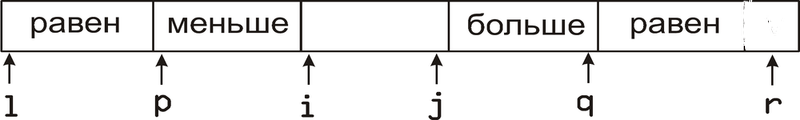
\includegraphics[width=0.6\textwidth]{1.png}
\end{figure}

Допустим, двигая i перегородку встречаем элемент меньше. Тогда все хорошо, просто сдвигаем ее направо на один. Если встречаем элемент равный, то делаем свап с самым левым меньшим, сдвигаем p и i перегородку вправо на один. Если встречаем элемент больший, то меняем его с левым меньшим. сдвигаем i перегородку вправо на один, меняем наш больший с левым равным элементом из правой области, сдвигаем p перегородку вправо на один, сдвигаем q перегородку вправо на один. 
Видно, что проходя каждый элемент массива будет выполняться не больше 5 операций. Значит сложность данного partition $O(n)$. Понятно, что быстрее чем за линейное время работать тоже не может. Тогда получаем $\Theta(n)$.


\section*{Задача №6}
Рассмотрим сумму, где $x_m$ - медиана. $x_{1...m - 1}$ меньше медианы, $x_{m + 1...2n - 1}$ больше медианы.
\[ |x_1 - s| + |x_2 - s| + ... + |x_m - s| + ... + |x_{2n} - s| + |x_{2n + 1} - s| \]
Пусть если $s$ равно медиане, то слагаемые равны 
\[ i_1 + i_2 + ... + 0 + ... + i_{2n} + i_{2n + 1} = A \] 
Теперь, если $s = m + \varepsilon$, где $\varepsilon > 0$, то
\[ i_1 + \varepsilon + i_2 + \varepsilon + ... + \varepsilon + ... + i_{2n} - \varepsilon + i_{2n + 1} - \varepsilon = A + \varepsilon \] 
Видно, что сумма будет больше. Мы доказали, что при $s = m$ сумма будет минимальной. А из предыдущих заданий ее мы можем найти за линейное время.
\end{document}